\chapter{Výsledky}
Zkoumali jsme dvojice molekul $\mathrm{BeH/BeH^-}$ a $\mathrm{OH/OH^-}$, protože se jedná o 
molekuly, které mají vázaný jak základní stav, tak anion, a zároveň se jedná o 
dostatečně malé systémy, aby bylo možné provádět výpočty přesnými metodami.

Ke kvantově chemickým výpočtům jsme používali balík výpočetně chemických programů 
MOLPRO.\cite{MOLPRO-WIREs, MOLPRO}.
CAS-SCF výpočty jsme prováděli pomocí programu MULTI \cite{WK85,KW85}, MRCI výpočty 
pomocí programu CI \cite{KW92} a FCI výpočty pomocí programu FCI \cite{KH84,KH89}.

U referenčních výpočtů jsme pro několik desítek mezijaderných vzdálenost vypočítali 
energii základního stavu molekul pro fixovaná jádra. Ze znalosti těchto křivek jsme 
poté zjišťovali parametry molekul, které je 
možné nalézt experimentálně, což jsou disociační energie aniontu i neutrální molekuly 
a 
elektronové afinity molekuly  ve vázaném stavu i asymptotickou elektronovou afinitu, 
která odpovídá 
elektronové afinitě některého z prvků v molekule.  Protože ale experimentální 
data nejsou určená minimem potenciální energie molekuly, ale základní vibrační 
hladinou, bylo třeba získat vibrační energetické hladiny dané molekuly metodou uvedenou 
v části \ref{te_vibr}. Počet geometrií, pro které jsme 
prováděli kvantově-chemické výpočty byl nedostatečný pro další numerické výpočty, a 
tedy jsme získané hodnoty proložili kubickým splinem, ze kterého jsme pak 
interpolovali hodnotu potenciálu v několika stovkách bodů. Poté jsme numericky získali 
energetické vibrační hladiny. Toto jsme opakovali pro různé kombinace báze, metoda.

Při hledání popisu targetu jsme nejprve získali křivky stavů neutrální molekuly jdoucí 
k několika nejnižším asymptotám pomocí přesnější metody ve velké bázi, kterou jsme 
použili jako referenční. Poté jsme tytéž stavy získali méně náročnou metodou, které 
jsme přeložili do grafu přes sebe. Křivky jsme veritikálně posunuli tak, aby byla 
totožná mimima základního stavu u zkoumané metody a referenčního výpočtu. Poté jsme 
vizuálně vybrali metodu nejlépe aproximující referenční výpočet.

\section{BeH}

Základní stav BeH je $^2\Sigma^+$, $\mathrm{BeH}^-$ je pak $^1\Sigma^+$, a v asymptotě 
jdou ke stavům $\mathrm{Be}(^1S) + \mathrm{H}(^2S)$, 
anion jde pak k $\mathrm{Be}(^1S) + \mathrm{H^-}(^1S)$.

Asymptotické chování excitovaných stavů je v tabulce \ref{taBeHas}, kde je popsáno asymptotické chování pomocí atomových stavů, energie asymptoty, oproti té nejnižší a molekulové stavy, které se k dané asymptotě limitně blíží.

\begin{table}
\centering
\caption{Asymptotické chování excitovaných stavů}
\bigskip
\label{taBeHas}
\begin{tabular}{ccc}
\toprule
asymptota & energie asympt. & molekulové stavy \\ 
\midrule
$\mathrm{Be}(^1\mathrm{S}) + \mathrm{H}(^2\mathrm{S})$ & $0.00$ & $^2\Sigma^+$ \\ 
$\mathrm{Be}(^3\mathrm{P}) + \mathrm{H}(^2\mathrm{S})$ & $2.725$ & $^2\Sigma^+,^4\Sigma^+,^2\Pi,^4\Pi$ \\
$\mathrm{Be}(^1\mathrm{P}) + \mathrm{H}(^2\mathrm{S})$ & $5.277$ & $^2\Sigma^+,^2\Pi$ \\ 
$\mathrm{Be}(^3\mathrm{S}) + \mathrm{H}(^2\mathrm{S})$ & $6.457$ & $^2\Sigma^+,^4\Sigma^+$ \\
$\mathrm{Be}(^1\mathrm{S}) + \mathrm{H}(^2\mathrm{S})$ & $6.779$ & $^2\Sigma^+$ \\
$\mathrm{Be}(^1\mathrm{D}) + \mathrm{H}(^2\mathrm{S})$ & $7.053$ & $^2\Sigma^+,^2\Pi,^2\Delta$ \\
$\left[\mathrm{Be}(^3\mathrm{P}) + \mathrm{H}(^2\mathrm{S})\right]$ &$[7.304]$& \\
\bottomrule
\end{tabular}
\end{table}

Při disociaci aniontu záporný náboj zůstává na vodíku, protože berylium má 
zápornou elektronovou afinitu.

\subsection{Referenční výpočty}
 Příklady křivek potenciální energie jsou vyobrazeny na obrázku  
\ref{VibrBeH1} spolu se základními vibračními hladinami neutrální molekuly i aniontu.
Křivky v tomto obrázku byly získány metodou FCI v bázi aug-cc-pVTZ.

Podobně jsme  získali elektronovou afinitu molekuly v disociovaném i nedisociovaném 
stavu a disociační energie molekuly i jejího aniontu, které pak můžeme srovnat s 
hodnotami získanými pomocí experimentu. Výsledné hodnoty jsou v tabulce \ref{beh1}

Metodou CI je v tabulkách myšlena metoda MRCI,za níž je uveden použitý aktivní prostor, 
zapsaný počtem jednotlivých molekulových orbitalů v dané ireducibilní reprezentaci pro grupu 
 $C_{2v}$ v pořadí $A_1, B_1, B_2, A_2$. Pro každou metodu je pak za lomítkem uvedena použitá báze.

Experimentální hodnotu disociační energie neutrální molekuly jsme získali 
z \cite{BeH-LeRoy}, její elektronovou afinitu pak z \cite{BeH-ElAf}. Elektronová 
afinita atomárního vodíku je pak známa velmi přesně, 
najít lze například v \cite{H-ElAf}. Disociační energie aniontu jsme 
v literatuře nenalezli, ale dané experimentální hodnoty jsou lineárně závislě, 
lze ji dopočítat pomocí
\begin{equation}
D(\mathrm{AB^-}) = D(\mathrm{AB}) + E_{ea}(B) - E_{ea}(AB),
\end{equation}

za předpokladu, že náboj zůstává na atomu B. Takto získanou hodnotu uvádíme v tabulce v závorce.

Nejnižší získané vibrační hladiny jsou pak v tabulce \ref{beh_vibr}.
Experimentální hodnoty jsou převzaty z \cite{BeH-LeRoy}.

\begin{figure}
\centering
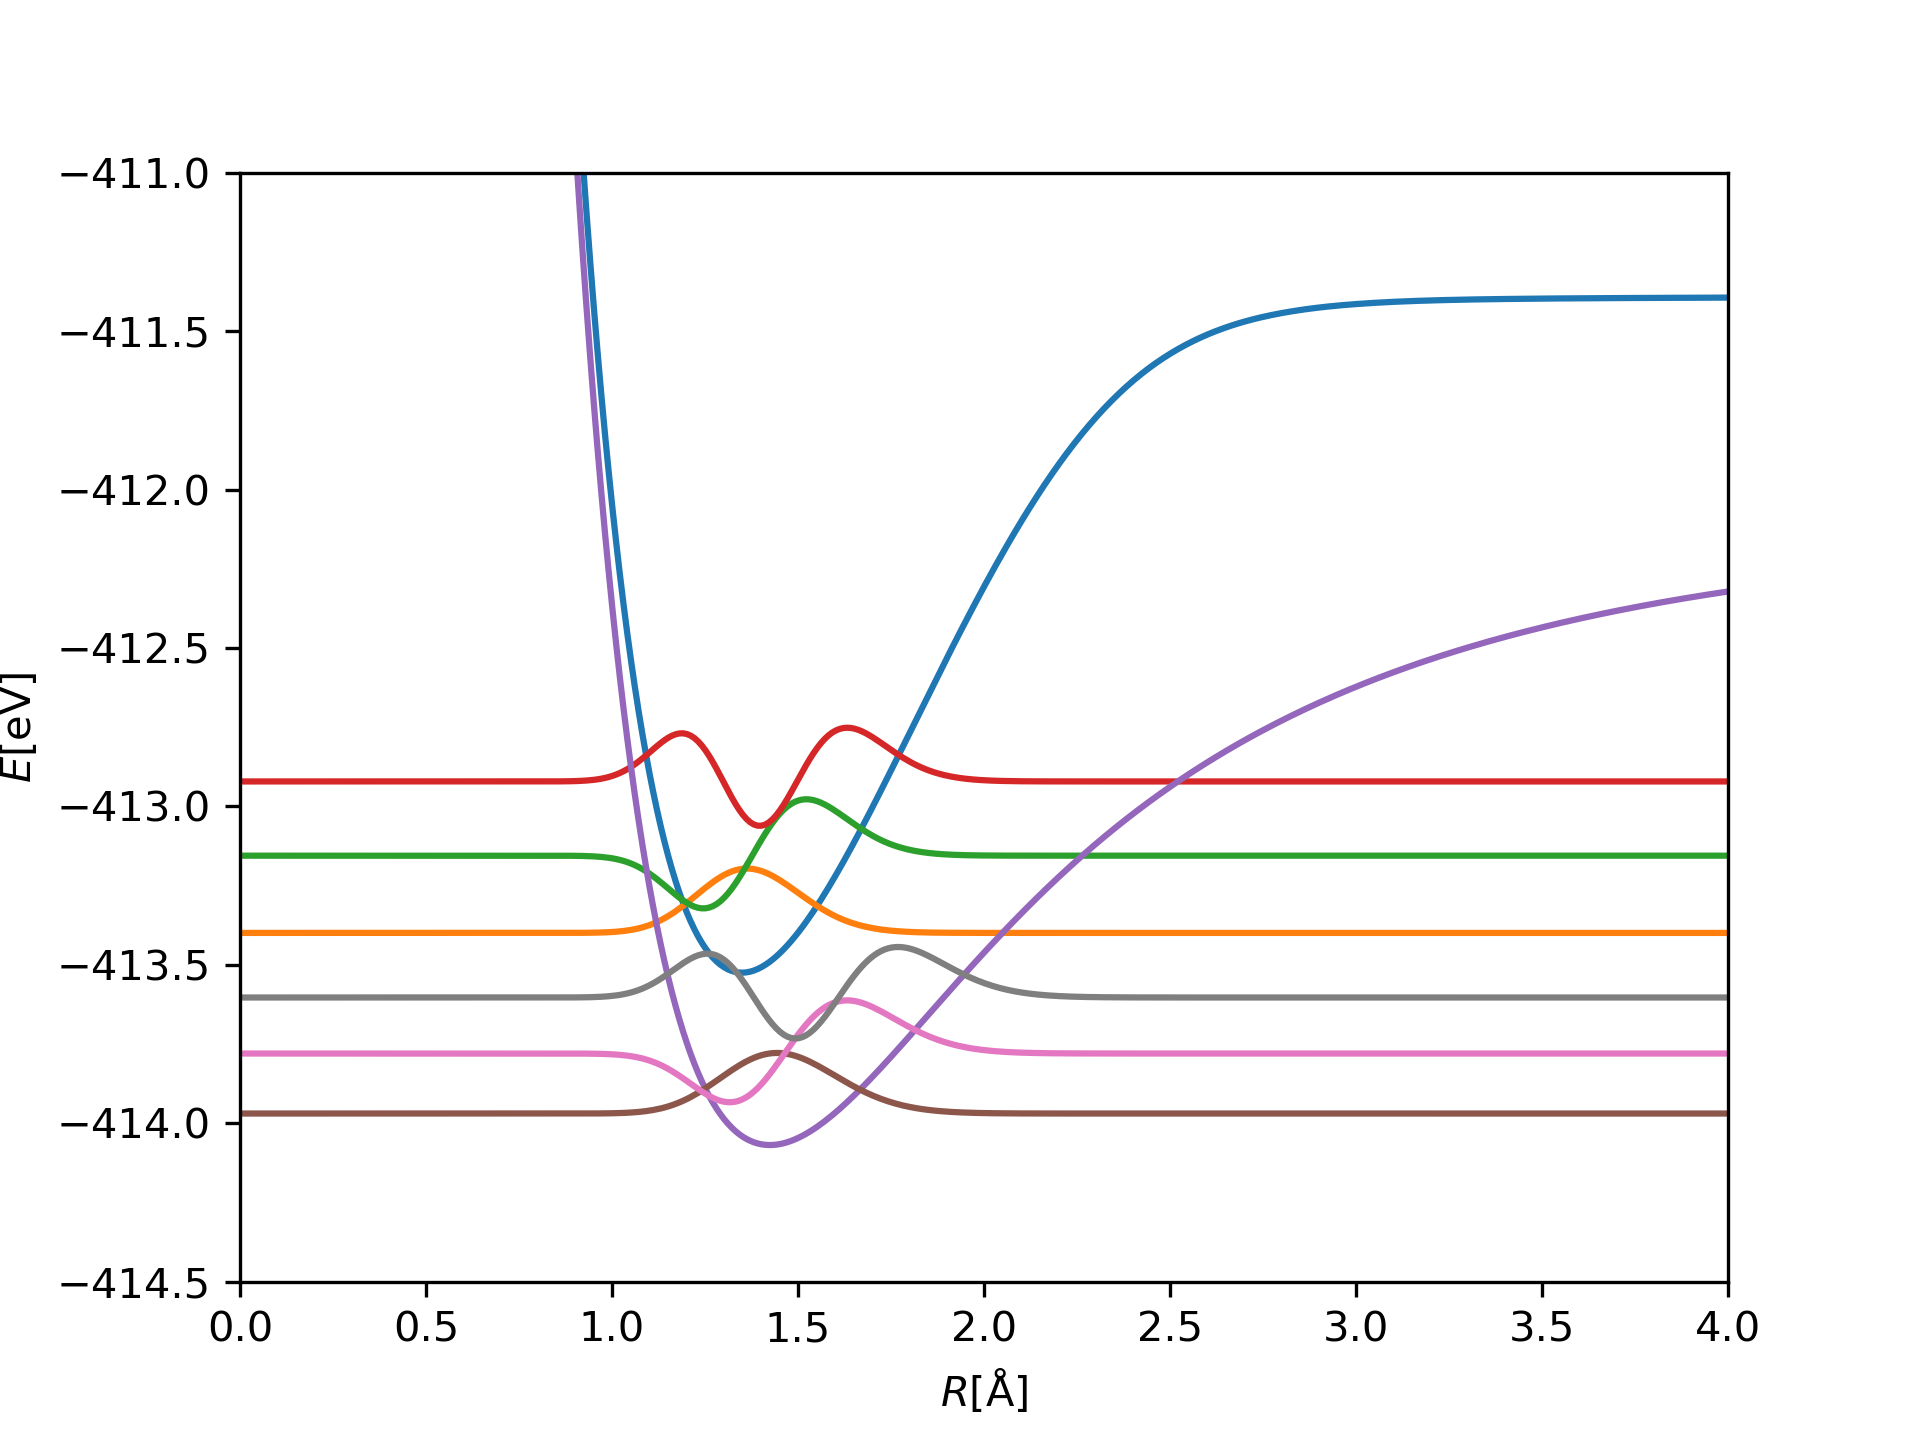
\includegraphics[width=0.8\textwidth]{../img/BeH-vibr1.png}
\caption{Potenciálové křivky základního stavu a nejnižší vibrační hladiny molekul $\mathrm{BeH/BeH^-}$}
\label{VibrBeH1}
\end{figure}
\ltable{../tbl/BeH.tex}{Některé získané měřitelné vlastnosti molekul $\mathrm{BeH/BeH^-}$}{beh1}
\htable{../tbl/BeH-vibr.tex}{Nejnižší čtyři vibrační hladiny molekuly $\mathrm{BeH}$}{beh_vibr}

Je vidět, že některé veličiny, především elektronová afinita se výrazně liší od 
experimentu. Konkrétně u experimentální hodnoty afinity je poměrně velká odchylka, 
navíc výpočty uvedené v \cite{KoputBeH, Koput_BeHan}, se s ostatními experimentálními hodnotami 
shodují, ale pro afinitu uvádí hodnotu $0.574\;\mathrm{eV}$, která je dosti vzdálená 
experimentální hodnotě, ale je v dobré shodě s našimi výsledky. Proto lze 
K dosažení ostatních experimentálních hodnot ovšem museli použít výrazně větší bázi a 
metodu která je size konzistentní a provést korekci na Bohrovu-Oppenheimerovu 
aproximaci. 

Na druhou stranu, pro použití v R-maticových výpočtech je třeba, aby metoda dávala   
především pro všechny geometrie dostatečně přesný rozdíl energie neutrální molekuly a 
aniontu. Vzhledem k tomu, že ve velikých bázích dosahujeme s docela dobrou 
přesností experimentální elektronové afinity i asymptoticky a v rovnovážné geometrii 
dosahujeme výše zmíněné hodnoty získané velmi přesnými výpočty. lze předpokládat, že 
chyby v energii neutrální molekuly a aniontu se odečtou a jejich rozdíl bude 
dostatečně přesný. \? Graf k tomu \?

Vibrační hladiny sice jsou blízko experimentálním hodnotám, ale nelze je použít pro 
rozlišení vhodnosti metody pro referenční výpočet, protože odchylka většiny metod se 
zdá být podobná.
 protože naše metoda jejich výpočtu, která používá aproximaci prvního řádu druhé 
derivace ve Shrödingerově rovnici, není pro tento účel dost přesná, navíc, jak plyne 
z \cite{Koput_BeH}, je pro získání třeba vyšší použitá teorie.
Nejlépe z těchto výpočtů sice vychází metoda CCSD(T), která ovšem špatně popisuje 
molekuly pro mezijaderné vzdálenosti v přechodu mezi rovnováhou a asymptotou.
To je pro naší aplikaci podstatné a proto se tato metoda pro referenční výpočet příliš 
nehodí.

\subsection{Popis targetu}
Ačkoliv lze pro takto malý systém použít metodu FCI se zamrznutým nejnižším molekulovým 
orbitalem, jak lze najít například v \cite{BeH-Rmat}, jedná se o časově náročný 
výpočet. Proto jsme se pokusili najít metodu CAS-SCF s takovými parametry, aby 
dostatečně dobře reprodukovala hodnoty získané přesnějšími metodami, protože by výrazně 
zkrátila R-maticový výpočet.
Prvně jsme provedli výpočet metodou FCI s 1 zamrznutým orbitalem, v bázi aug-cc-pVTZ, 
který jsme použili jako referenční. Tentýž výpočet jsme provedli i s bází aug-cc-pVDZ, 
přičemž srovnání je na obrázku \ref{gr_Beh_FCI}. Z něj vidíme, že od stavů s rozdílem 
od základního stavu vyšším než cca 6 eV selhává popis pomocí aug-cc-pVDZ báze, a tedy 
přesnost metod nad touto úrovní nemá smysl uvažovat, neboť větší báze již nelze v R-
maticových výpočtech použít kvůli výpočetní náročnosti. Je vidět, že i metoda FCI se na 
některých místech chová špatně, především kvůli velkému množství blízkých stavů, 
přičemž se nám nedařilo zvolit počet stavů tak, aby se nějaký vyšší, který jsme již 
neuvažovali, nezasahoval do již zvolených stavů. U metody FCI to nedělalo tak výrazné 
potíže s výjimkou některých zlomů a přeskakování ve vyšších excitovaných stavech, ale  
nepodařilo se nám kvůli tomu provést výpočet metodou MRCI, který by uvažoval tyto 
excitované stavy.

Zkusili jsme srovnat několik metod CAS-SCF v aug-cc-pVDZ bázi lišících se aktivním 
prostorem a zjistili, že v okolí rovnovážné vzdálenosti popisuje molekulu CAS-SCF s 
aktivním prostorem $6,2,2,0$, které je zobrazeno na obrázku \ref{gr_Beh_6220} spolu s 
referenčním FCI v aug-cc-pVTZ bázi na pozadí šedou barvou. Zmenšeni, ale paradoxně i 
zvětšení aktivního prostoru vedlo k výraznému zhoršení chování křivek, jak je zřejmé z 
obrázků \ref{gr_Beh_5220} a \ref{gr_Beh_8330}. Ve všech uvedených výpočtech jsme 
nechali zamrznutý nejspodnější orbital, ale jeho nezamrznutí téměř nemělo vliv na 
výsledek, 
což jsme zkoušeli u prvního zmíněného CAS-SCF výpočtu.

V okolí rovnovážné geometrie první zmíněná metoda CAS-SCF popisuje velmi dobře křivky 
získané metodou FCI pro stavy s energií do 6 eV nad základním stavem, kde začíná 
selhávat použitá báze. Pro větší mezijaderné vzdálenosti pak metoda nedává dobré 
výsledky, ale to je obecný problém CAS-SCF metod a v R-maticových výpočtech nedělá 
tento jev až tak velké potíže.

\begin{figure}
\centering
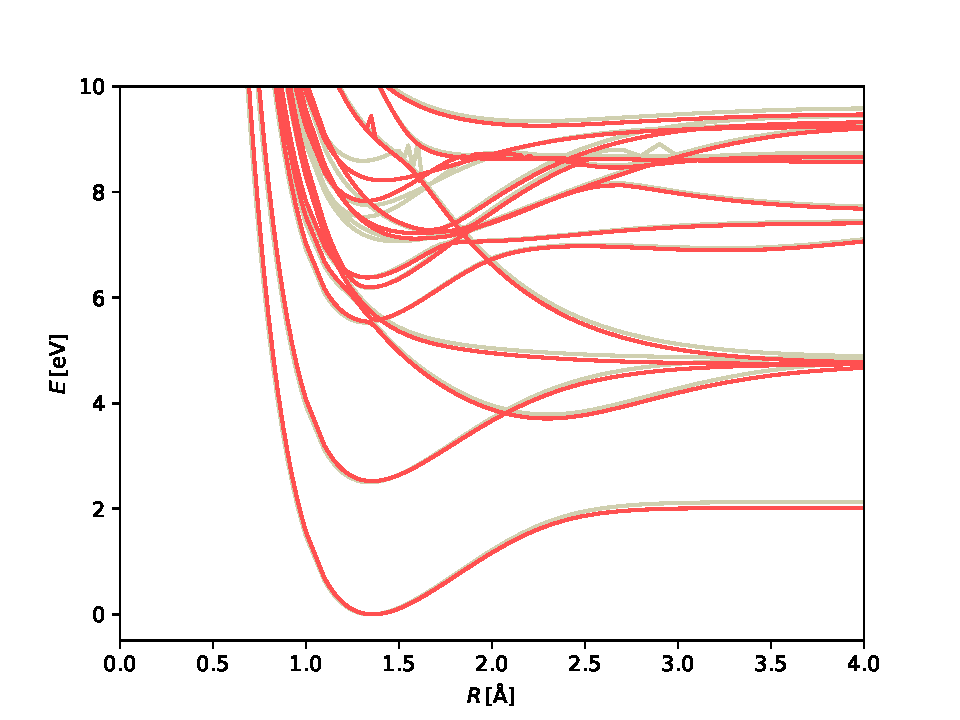
\includegraphics[width=0.8\textwidth]{../img/BeH-FCI-DZ.pdf}
\caption{Srovnání metody FCI pro neutrální molekulu BeH v bázi aug-cc-pVDZ (červená) a referenčním FCI v bázi aug-cc-pVTZ (šedá)}
\label{gr_Beh_FCI}
\end{figure}

\begin{figure}
\centering
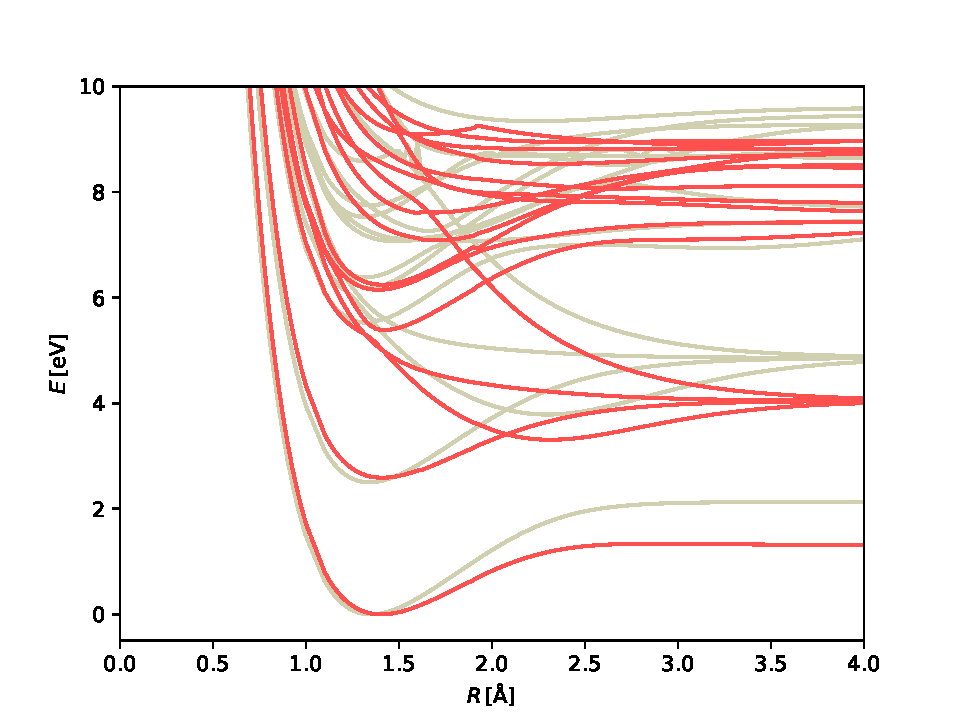
\includegraphics[width=0.8\textwidth]{../img/BeH-MULTI-DZ-6220.pdf}
\caption{Srovnání CAS-SCF výpočtu s aktivním prostorem $6,2,2,0$ v aug-cc-pVDZ bázi s referenčním FCI}
\label{gr_Beh_6220}
\end{figure}

\begin{figure}
\centering
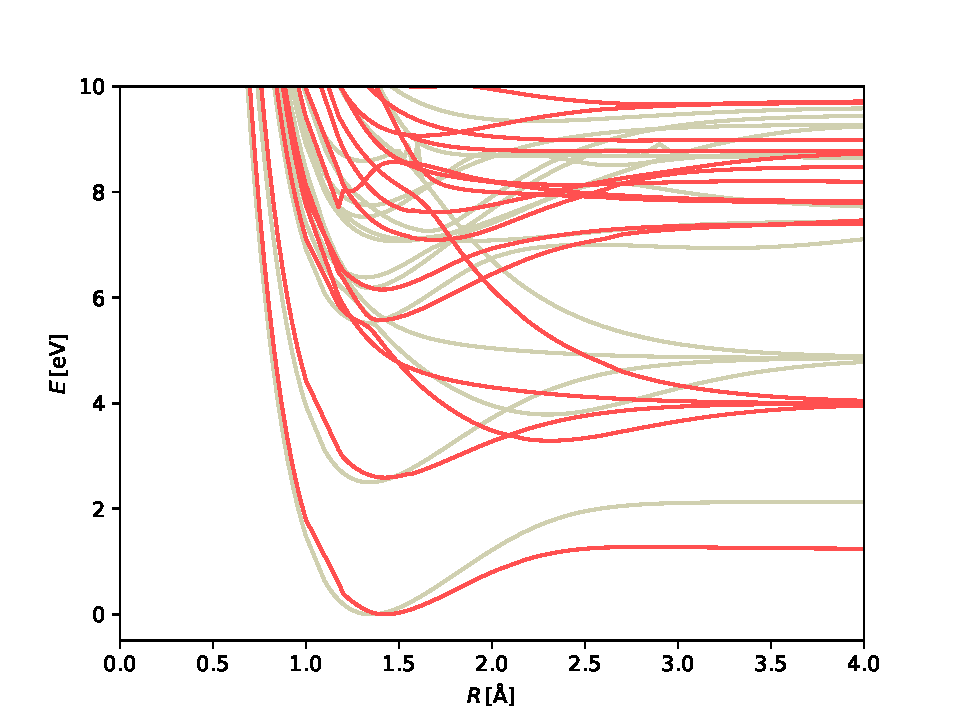
\includegraphics[width=0.8\textwidth]{../img/BeH-MULTI-DZ-5220.pdf}
\caption{Srovnání CAS-SCF výpočtu s aktivním prostorem $5,2,2,0$ v aug-cc-pVDZ bázi s referenčním FCI}
\label{gr_Beh_5220}
\end{figure}

\begin{figure}
\centering
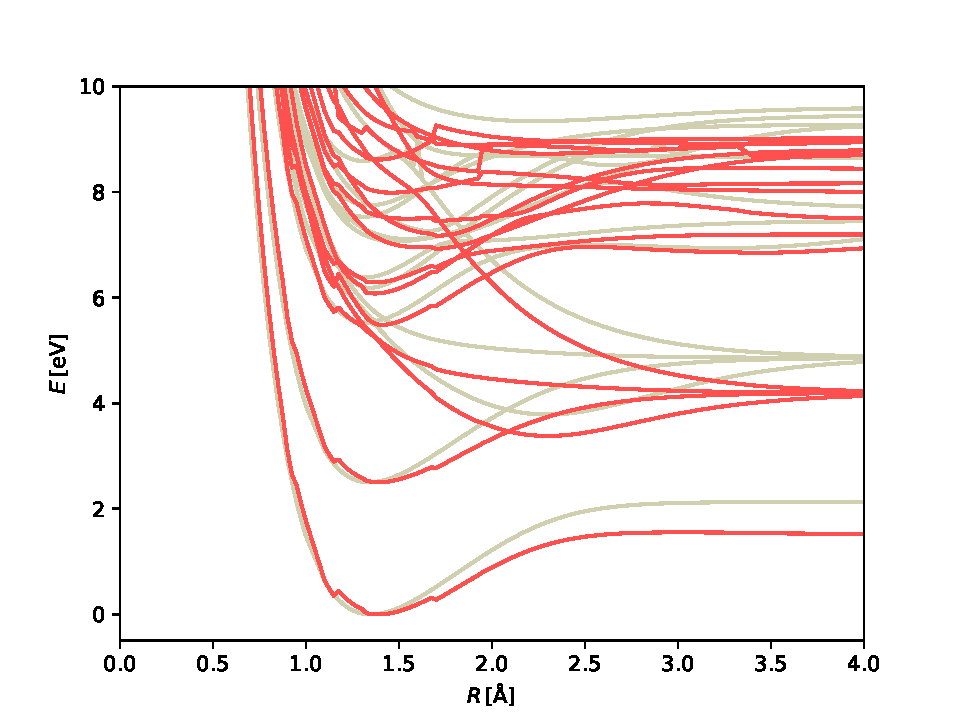
\includegraphics[width=0.8\textwidth]{../img/BeH-MULTI-DZ-8330.pdf}
\caption{Srovnání CAS-SCF výpočtu s aktivním prostorem $8,3,3,0$ v aug-cc-pVDZ bázi , s referenčním FCI}
\label{gr_Beh_8330}
\end{figure}

\section{OH}
Základní stav molekuly OH je $\mathrm{^2\Pi}$ s asymptotou 
$\mathrm{O}(^3p) + \mathrm{H}(^2s)$. Další 
stavy jdoucí k této asymptotě jsou $\mathrm{^4\Pi, ^4\Sigma^-, ^2\Sigma^- }$.
Nejnižší asymptoty neutrální molekuly jsou pak v tabulce \ref{taOHas}, v závorce je
nejnižší asymptota, kterou jsme neuvažovali.

 Anion je v základním stavu $^1\Sigma^+$, s asymptotou
  $\mathrm{O^-}(^2\mathrm{P}) + \mathrm{H}(^2\mathrm{S})$. 
  K této asymptotě jdou ještě stavy
  $\mathrm{^3\Sigma^+,^1\Pi, ^3\Pi}$
 Pod asymptotou základního stavu leží i asymptota 
 $\mathrm{O}(^3\mathrm{P}) + \mathrm{H^-}(^1\mathrm{S})$, 
 ke které jdou stavy $\mathrm{^3\Sigma^-, ^3\Pi}$.

\begin{table}
\centering
\caption{Asymptotické chování nejnižších stavů neutrální molekuly OH}
\label{taOHas}
\bigskip
\begin{tabular}{ccc}
\toprule
asymptota & energie asympt. & molekulové stavy \\ 
\midrule
$\mathrm{O}(^3\mathrm{P}) + \mathrm{H}(^2\mathrm{S})$ & $0.000$ & $\mathrm{^2\Sigma^-}, \mathrm{^4\Sigma^-},\mathrm{^2\Pi},\mathrm{^4\Pi}$ \\ 
$\mathrm{O}(^1\mathrm{D}) + \mathrm{H}(^2\mathrm{S})$ & $1.967$ & $\mathrm{^2\Sigma^+}, \mathrm{^2\Pi}, \mathrm{^2\Delta}$ \\ 
$\mathrm{O}(^1\mathrm{S}) + \mathrm{H}(^2\mathrm{S})$ & $4.190$ & $ \mathrm{^2\Sigma^+}$ \\ 
$[\mathrm{O}(^5\mathrm{S}) + \mathrm{H}(^2\mathrm{S})]$ & $[9.146]$ \\ 
\bottomrule
\end{tabular} 
\end{table}

\subsection{Referenční výpočty}
Pro různé metody jsme získali křivky neutrální molekuly i aniontu, z nich jsme získali
disociační energii energie aniontu i neutrální molekuly, i rovnovážnou a asymptotickou 
elektronovou afinitu neutrální molekuly. Získané hodnoty, spolu s experimentálními daty 
jsou v tabulce \ref{oh1}
Hodnotu disociační energie neutrální molekuly uvádí například \cite{CRC_Handbook90}, 
stejně jako elektronovou afinitu této molekuly i atomárního kyslíku.

Vibrační energetické hladin pro křivky neutrální molekuly, získané různými metodami 
jsou v tabulce \ref{oh_vibr}. Referenční hodnoty jsou použity hodnoty převzaté z 
\cite{OH_vibr}.

\begin{figure}
\centering
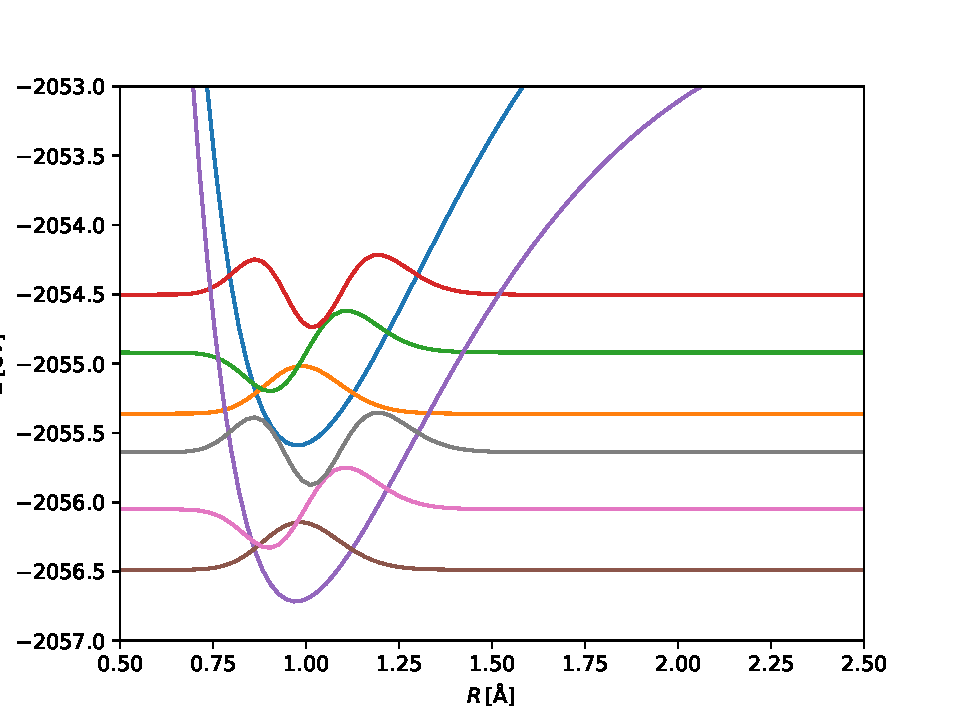
\includegraphics[width=0.8\textwidth]{../img/OH-vibr1.pdf}
\caption{Potenciálové křivky základního stavu a nejnižší vibrační hladiny molekul $\mathrm{OH/OH^-}$ \label{VibrOH1}}
\end{figure}

\ltable{../tbl/OH.tex}{Některé získané měřitelné vlastnosti molekul $\mathrm{OH/OH^-}$}{oh1}
\htable{../tbl/OH-vibr.tex}{Nejnižší čtyři vibrační hladiny molekuly $\mathrm{OH}$}{oh_vibr}
\htable{../tbl/OHan-vibr.tex}{Nejnižší čtyři vibrační hladiny molekuly $\mathrm{OH^-}$}{ohan_vibr}


\subsection{Popis targetu}
Pro popis targetu jsme jednak provedli výpočet křivek pro srovnání metodou MRCI s 
aktivním prostorem pro vstupní CAS-SCF 8,2,2,0 a bází aug-cc-pVQZ. Ukázalo se, stejně 
jako pro molekulu BeH, že z metod použitelných v rozptylových výpočtech dobře popisuje 
tuto molekulu CAS-SCF v bázi aug-cc-pVDZ s aktivním prostorem $6,2,2,0$. Křivky  
získané touto metodou, spolu s referenčními křivkami v pozadí jsou v grafu 
\ref{gr_OH_6220}. Na rozdíl od výpočtu touto metodou pro molekulu BeH je zde vidět 
nefyzikální nespojitost pro mezijadernou vzdálenost kolem $0.9\AA$. Tu jsme se 
pokusili odstranit nastavením různých vah pro různé stavy. K odstranění nespojitosti 
vedlo nastavení hodnoty váhy 0.5 na na oba degenerované stavy základní křivky $^2\Pi$ 
a váhy 1.0 na nejnižší stav  $^2\Sigma^+$. (Nejnižší vázaný excitovaný stav), s 
nulovou váhou na všech ostatních stavech.

V grafu \ref{gr_OH_7330_w} je pak výpočet s vahami jen na vázaných stavech podobně 
jako u předchozího zmíněného výpočtu a aktivním prostorem $7,3,3,0$. Ten vykazuje 
nepatrně lepší výsledky pro zmíněný první excitovaný stav, ale za cenu většího 
aktivního prostoru a tím pádem i větší výpočetní náročnosti. Ale u tohoto výpočtu se 
výrazně rozchází asymptotická energie pro stavy jdoucí k prostřední asymptotě, která 
by správně měla být degenerovaná.

\begin{figure}
\centering
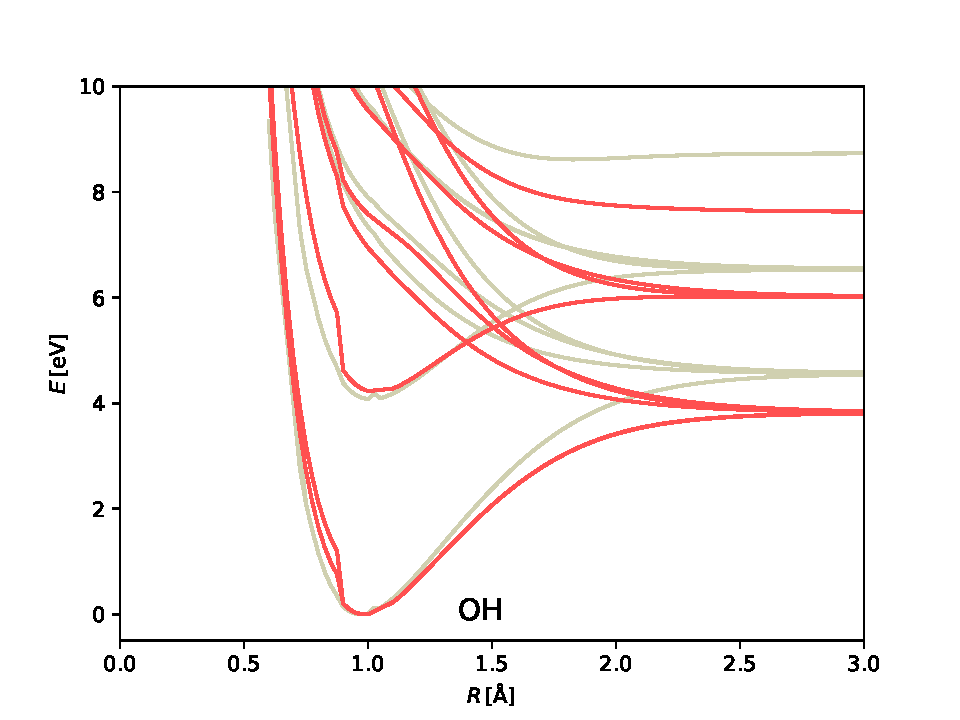
\includegraphics[width=0.8\textwidth]{../img/OH-MULTI-DZ-6220.pdf}
\caption{Srovnání CAS-SCF výpočtu s aktivním prostorem $6,2,2,0$ v aug-cc-pVDZ bázi 
s referenčním MRCI}
\label{gr_OH_6220}
\end{figure}

\begin{figure}
\centering
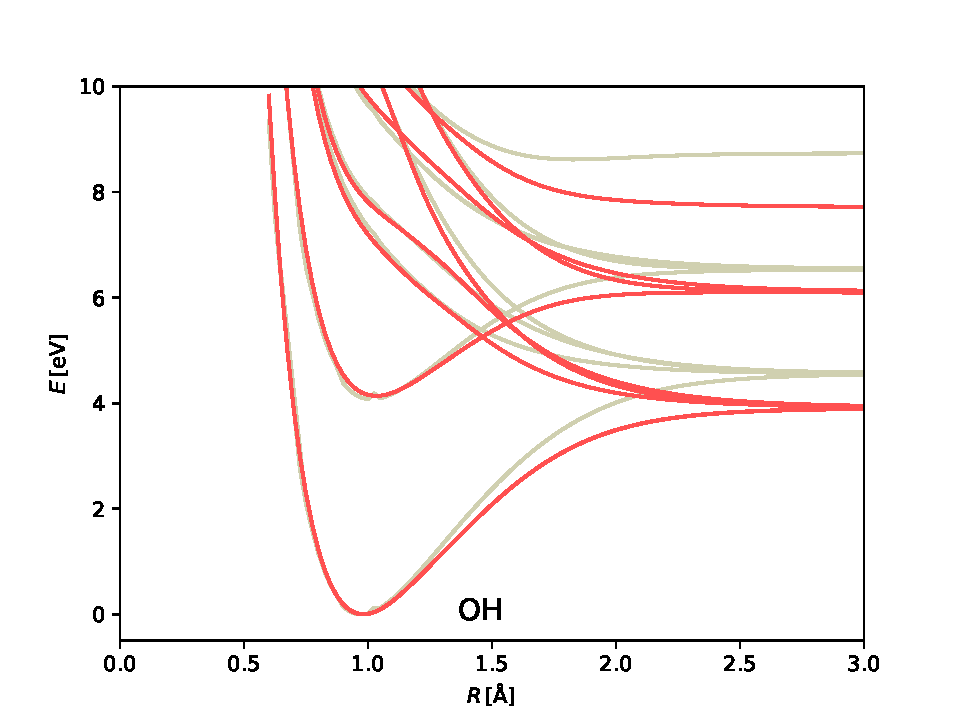
\includegraphics[width=0.8\textwidth]{../img/OH-MULTI-DZ-6220-w8.pdf}
\caption{Srovnání CAS-SCF výpočtu s aktivním prostorem $6,2,2,0$ v aug-cc-pVDZ bázi  a vahami jen na vázaných stavech s referenčním MRCI}
\label{gr_OH_6220_w}
\end{figure}

\begin{figure}
\centering
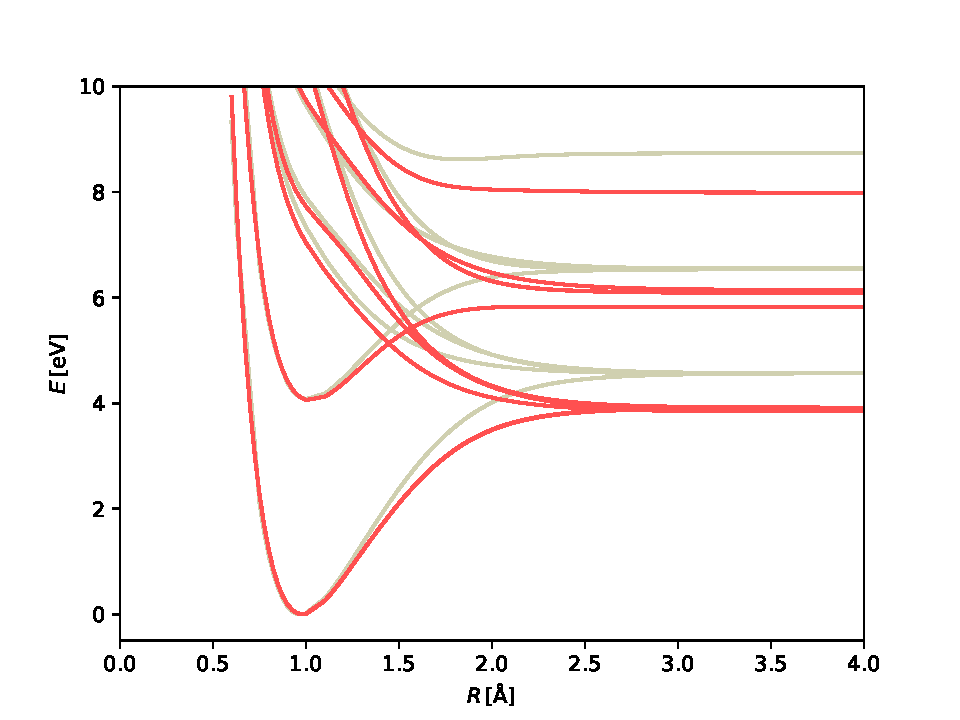
\includegraphics[width=0.8\textwidth]{../img/OH-MULTI-DZ-7330-w1.pdf}
\caption{Srovnání CAS-SCF výpočtu s aktivním prostorem $7,3,3,0$ v aug-cc-pVDZ bázi  a vahami jen na vázaných stavech s referenčním MRCI}
\label{gr_OH_7330_w}
\end{figure}